\section{服务与服务系统}

\subsection{服务}

\subsubsection{服务的概念}

\begin{itemize}
    \item 服务是为客户(担任协同提供者)所执行的非持久的,无形的体验。
    \item 服务是单个或一系列活动。这些活动或多或少带有无形的天然属性;这些活动通常(虽然不是必须)在客户和服务雇员/物理资源和产品/服务提供者的系统之间的交互中所发生。它们用来提供针对客户问题的解决方案。
\end{itemize}

服务的例子
\vspace{-0.8em}
\begin{multicols}{4}
    \begin{itemize}
        \item 传统物流仓储
        \item 信息咨询
        \item 金融、股票市场
        \item 租赁
        \item 科学技术服务
        \item 管理
        \item 娱乐
        \item ……  
    \end{itemize}
\end{multicols}
\vspace{-1em}

\subsubsection{服务与制造}

商品与服务的精确定义应根据其属性加以区分
\begin{itemize}
    \item 商品是可以创造和转让的有形实物或产品;它随着时间的推移而存在,因此可以在以后创建和使用。
    \item 服务是无形的,易变质的。它是同时或几乎同时创建和使用的事件或过程。虽然消费者在实际服务产生后无法保留,但服务的努力可以保留。
\end{itemize}

\begin{figure}[H]
	\setcounter{subfigure}{0}
	\centering
	\vspace{-0.5em}	
	\subfloat[Service vs.Manufacturing Model]{
	\begin{minipage}[c]{0.7\linewidth}
	\centering
	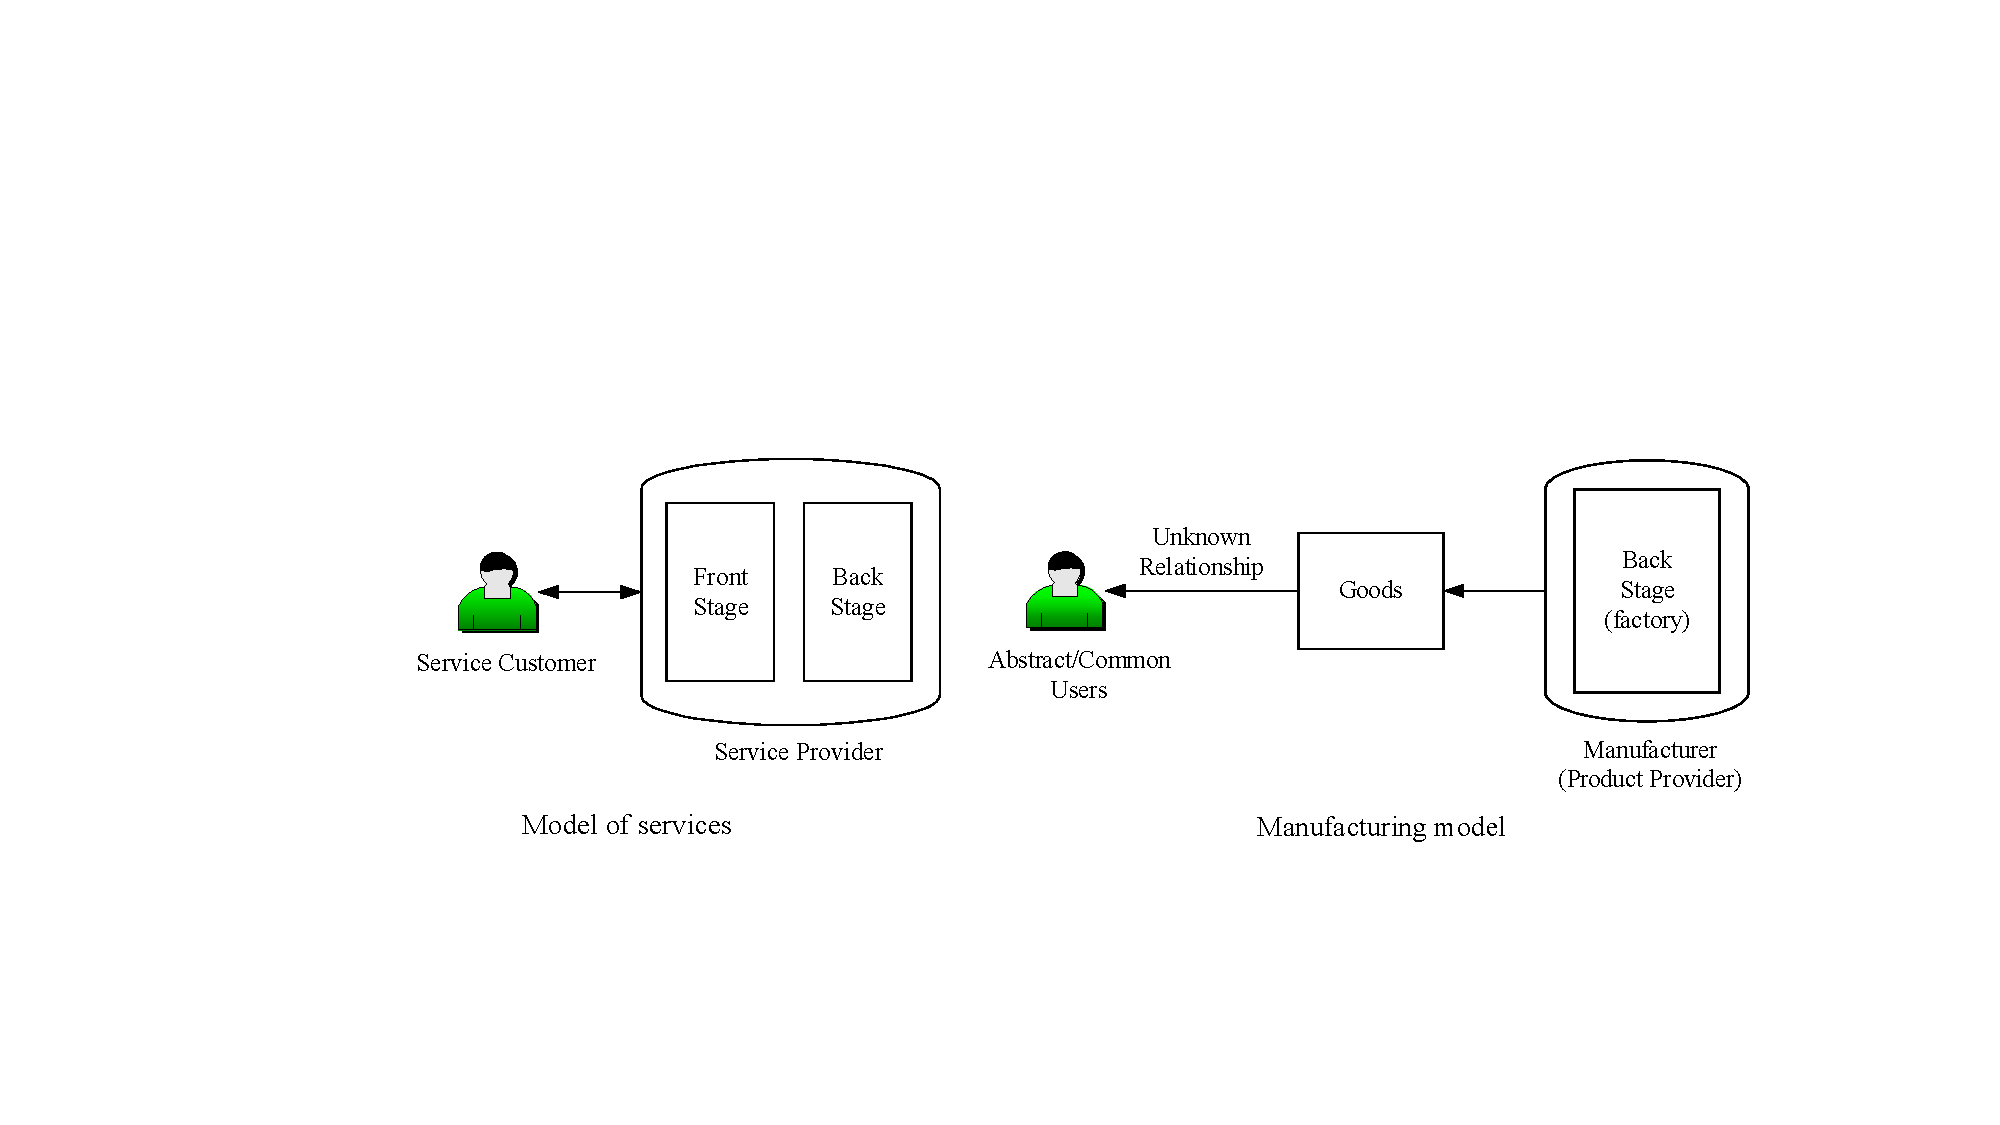
\includegraphics[width=0.97\linewidth]{images/Services vs Goods.pdf}
	\end{minipage}
	}
    \hfill
	\subfloat[Service-goods continuum]{
	\begin{minipage}[c]{0.25\linewidth}
	\centering
	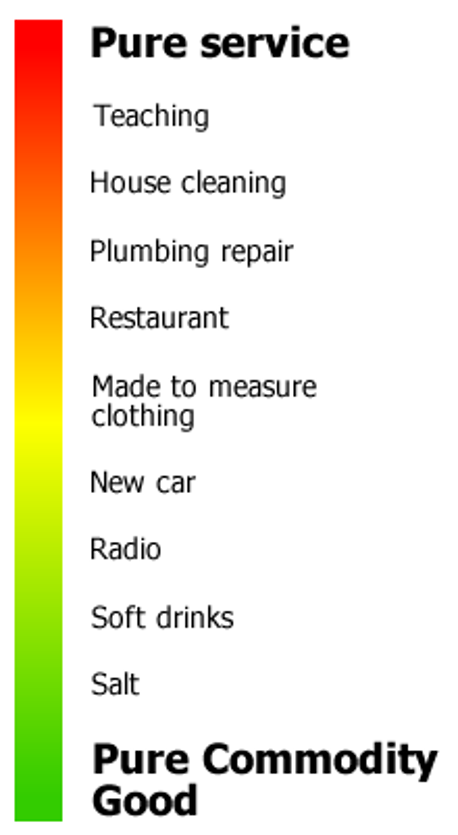
\includegraphics[width=0.9\linewidth]{images/Service-goods continuum.png}
	\end{minipage}
	}
	\centering
	\vspace{-1em}
\end{figure}

\subsubsection{服务发展趋势}
\vspace{-0.8em}
\begin{multicols}{2}
    \begin{itemize}
        \item 单纯的制造持续减少
        \item 服务产业持续增长
        \vspace{-0.8em}
        \begin{multicols}{3}
            \begin{itemize}
                \item 物业服务
                \item 安全保障
                \item 园艺
                \item 清洁工作
                \item 软件开发(外包)
            \end{itemize}
        \end{multicols}
        \vspace{-1.2em}
        \item 服务变得越来越复杂
        \begin{itemize}
            \item 银行的呼叫中心(业务支持系统)
            \item 提供医疗服务的医院(HIS)
            \item 复杂企业的管理(ERP, CRM, …)
            \item 电子银行或电子商务(B2C, B2B, …)
        \end{itemize}
        \item 引入各种IT系统
        \begin{itemize}
            \item 有没有服务雇员均可
        \end{itemize}
    \end{itemize}
\end{multicols}
\vspace{-1em}


\subsection{服务系统}

\subsubsection{基本概念}
服务系统是指用以实现业务服务的IT软件系统,相当多的软件系统是服务系统。

服务系统可以非正式定义为6元组
\vspace{-0.8em}
\begin{multicols}{3}
    \begin{itemize}
        \item 输入
        \item 输出
        \item 目标(内部目标,外部目标)
        \item 转换过程
        \item 组件
        \item 传感器
    \end{itemize}
\end{multicols}
\vspace{-1em}

其中组件包括
\vspace{-0.8em}
\begin{spacing}{1.12}
\begin{multicols}{2}
    \begin{itemize}
        \item 服务人员
        \vspace{-0.8em}
        \begin{multicols}{2}
            \begin{itemize}
                \item 设计人员
                \item 开发人员
                \item 测试人员
                \item ……
            \end{itemize}
        \end{multicols}
        \vspace{-1.2em}
        \item 服务伙伴
        \vspace{-0.8em}
        \begin{multicols}{2}
            \begin{itemize}
                \item 客户
                \item 服务雇员
            \end{itemize}
        \end{multicols}
        \vspace{-1.2em}
        \item 服务信息
        \item 服务步骤
        \item 服务基础架构资源架构(物理/IT/抽象)
    \end{itemize}
\end{multicols}
\end{spacing}
\vspace{-1em}

\begin{figure}[H]
	\setcounter{subfigure}{0}
	\centering
	\vspace{-0.5em}	
	\subfloat[Self Contained \& Encapsulated]{
	\begin{minipage}[c]{0.6\linewidth}
	\centering
	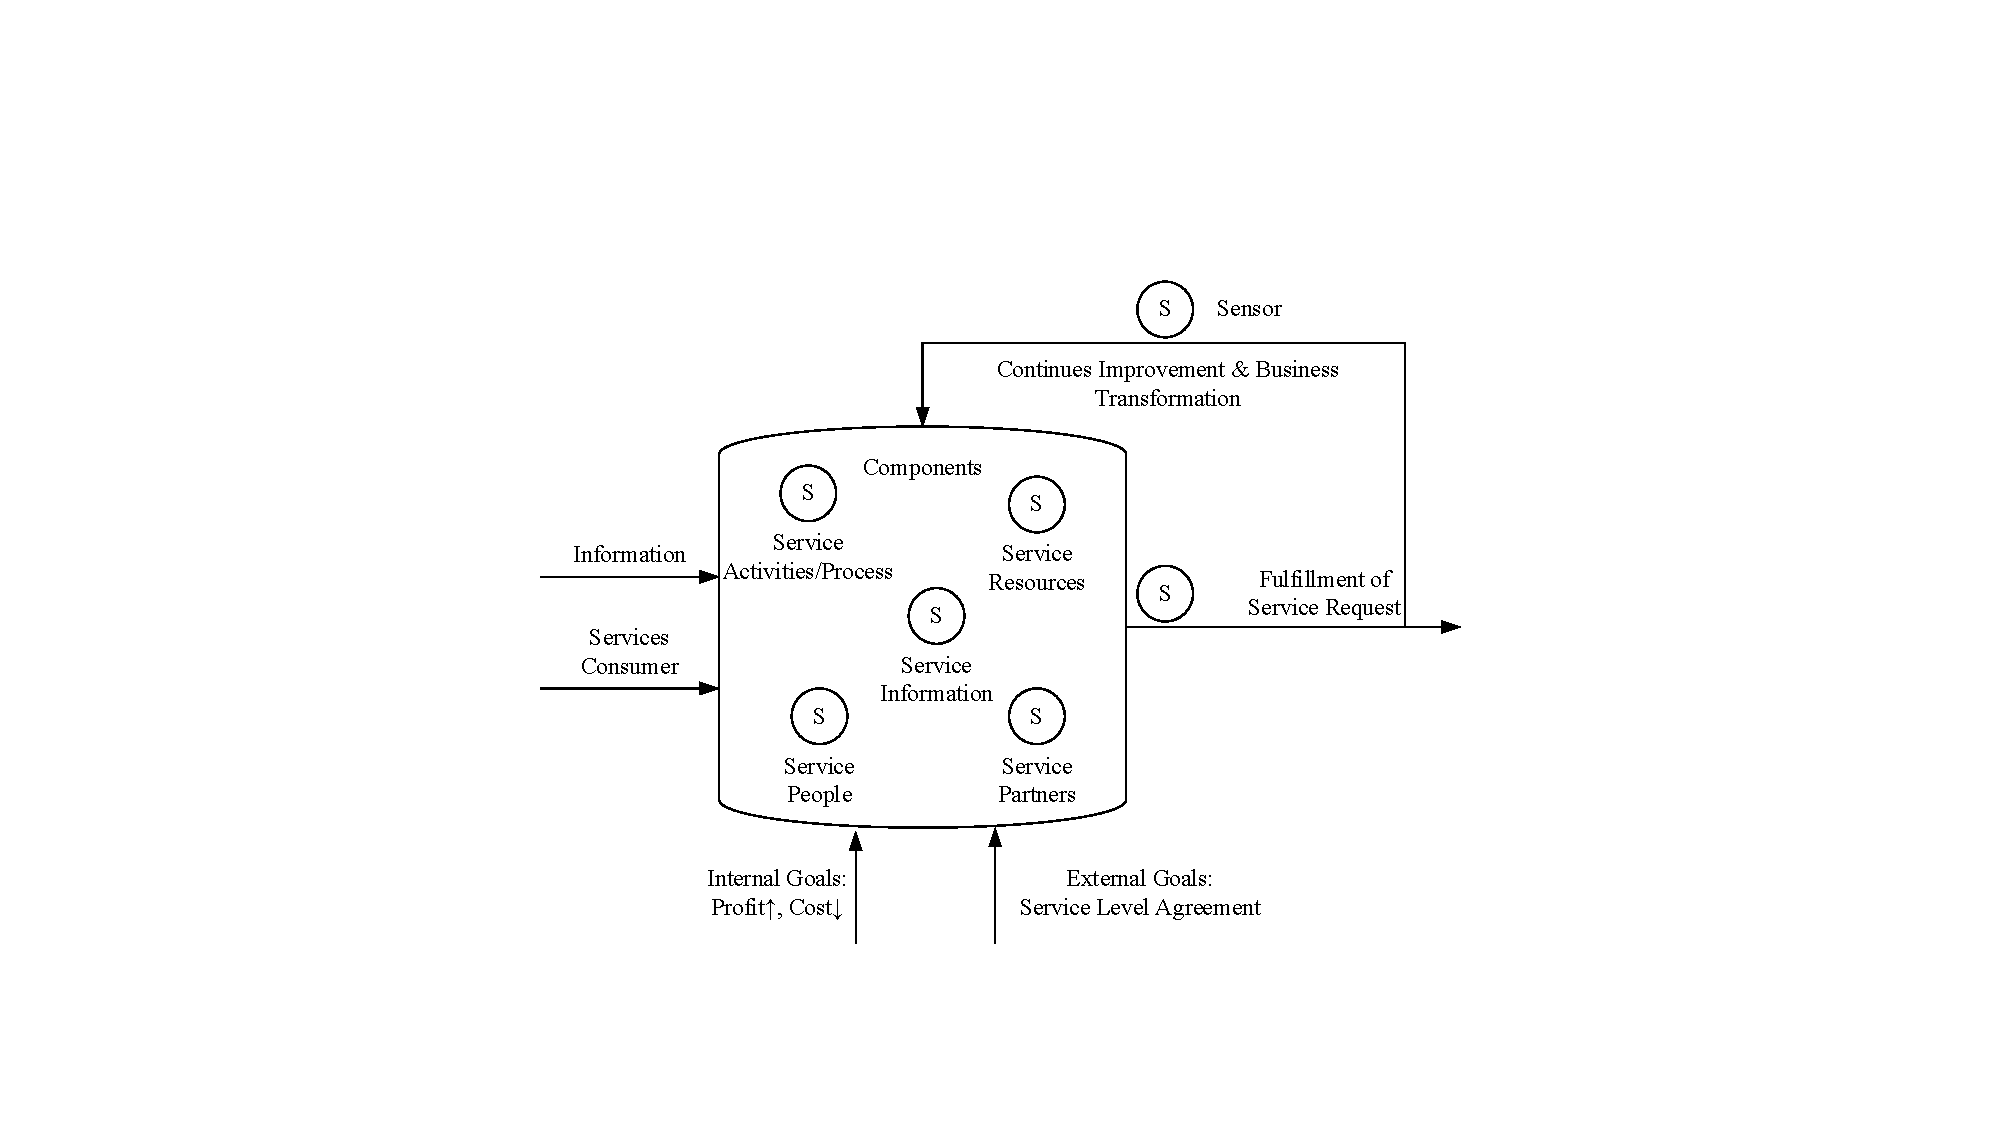
\includegraphics[width=0.97\linewidth]{images/Self Contained Encapsulated.pdf}
	\end{minipage}
	}
	\subfloat[服务系统的视角观点]{
	\begin{minipage}[c]{0.35\linewidth}
	\centering
	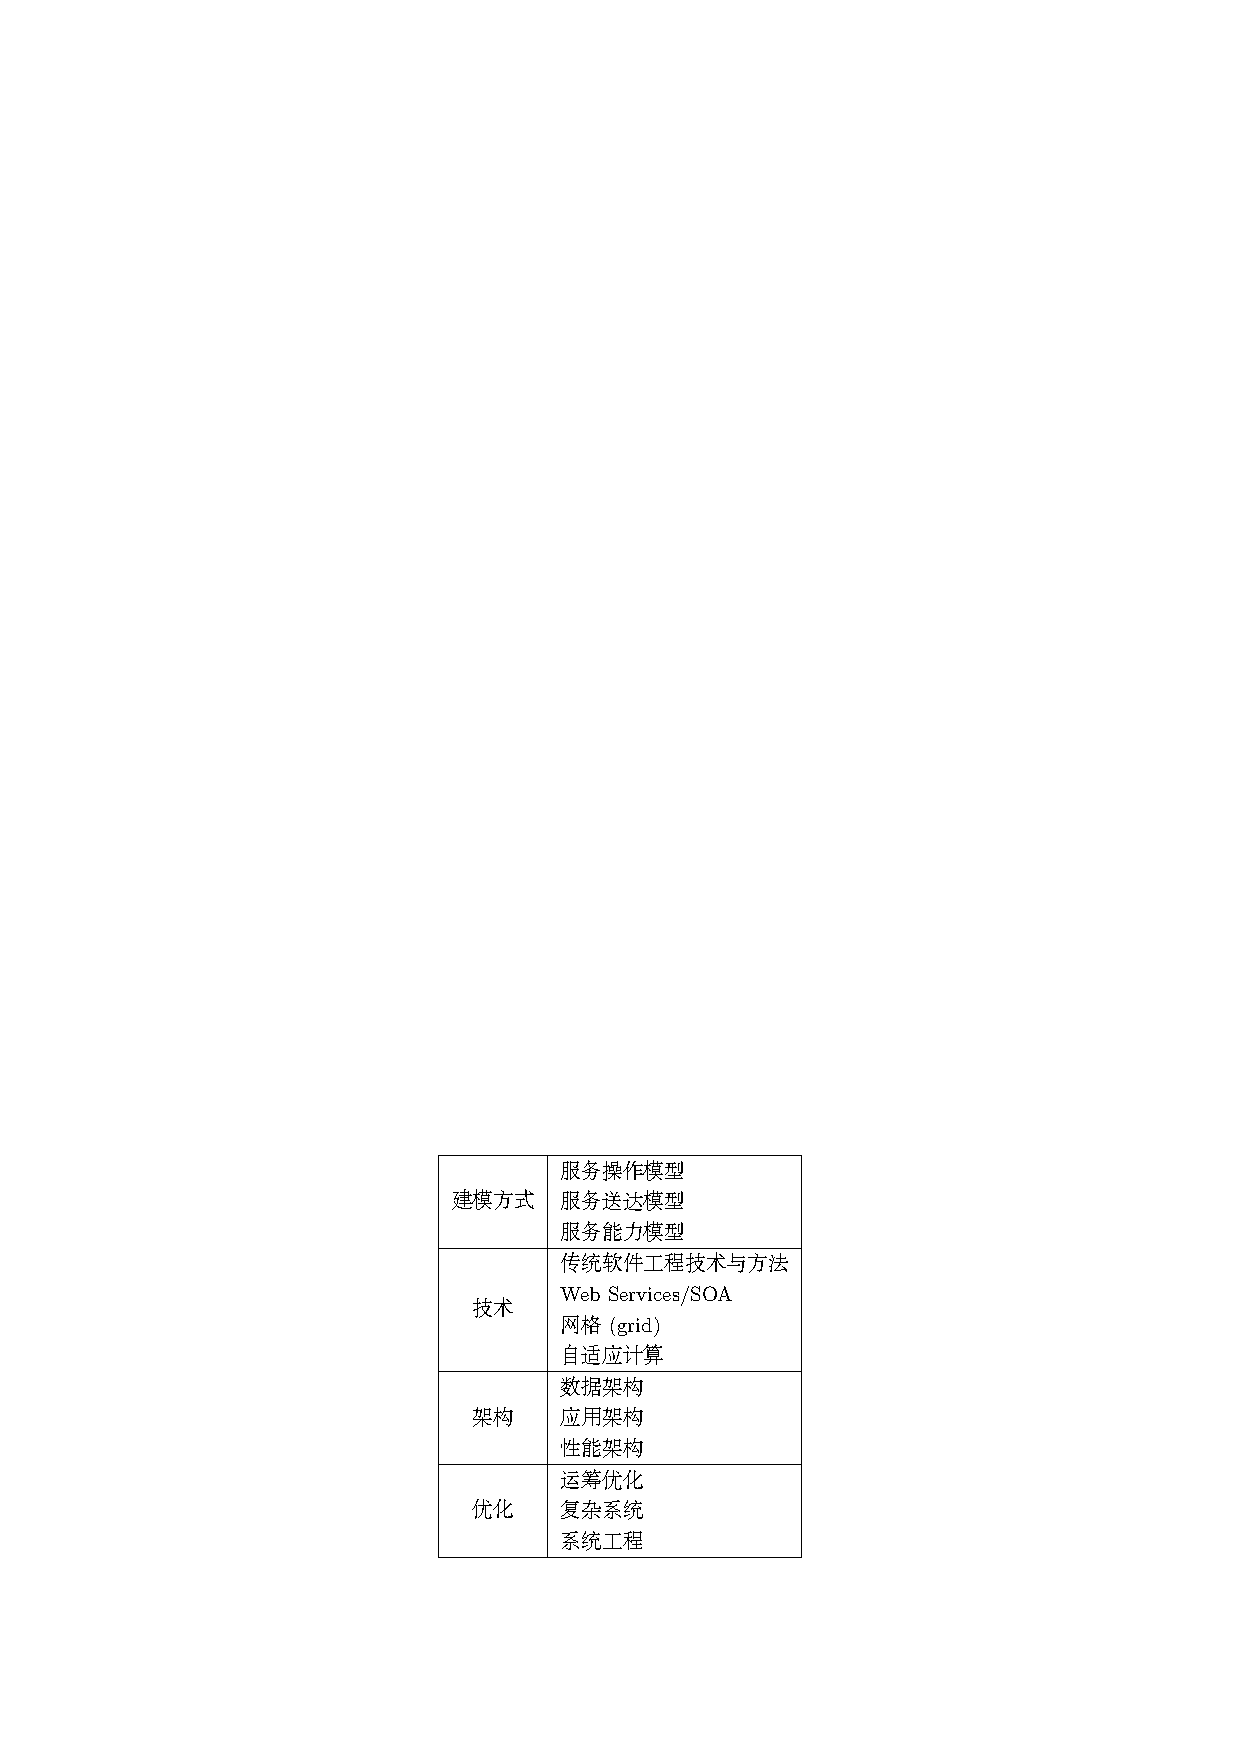
\includegraphics[width=0.97\linewidth]{images/服务系统的视角观点.pdf}
	\end{minipage}
	}
	\centering
	\vspace{-1em}
\end{figure}

服务系统遇到的问题和挑战
\vspace{-0.8em}
\begin{multicols}{2}
    \begin{itemize}
        \item 服务系统的复杂性
        \item 服务系统的灵活性
        \item 专业化和外包模式
        \item 计算环境的演化
        \item IT专家和业务专家之间的隔阂
        \item 新增价值和创新功能
        \item 一系列有着略微差异的服务系统(产品家族、产品线) 
    \end{itemize}
\end{multicols}
\vspace{-1em}

\subsubsection{IT使能的服务系统}
当业务服务由服务系统提供,该服务被称为IT使能的服务系统。

服务表示至少一个服务提供商和一个服务使用者之间为实现特定业务目标或解决方案目标而进行的基于关系的交互活动。

其中可能既含有IT服务,也可能含有非IT服务,区别包括:
\vspace{-0.8em}
\begin{multicols}{3}
    \begin{itemize}
        \item 关键绩效(KPIs)不同
        \item 需求管理不同
        \item 服务步调不同
    \end{itemize}
\end{multicols}
\vspace{-1em}

IT使能的服务系统具有2个特点:操作模型和收费模型

操作模型
\vspace{-0.8em}
\begin{multicols}{3}
    \begin{itemize}
        \item 点对点模型
        \item 集中服务模型
        \item 商务流程外包(BPO)
        \item 以数据为核心的外包(DCO)
        \item 通过在线经纪代理提供服务
    \end{itemize}
\end{multicols}
\vspace{-1em}

收费模型
\vspace{-0.8em}
\begin{multicols}{3}
    \begin{itemize}
        \item 免费模型
        \item 基于费用模式的模型
        \item 政府提供的公益模型
    \end{itemize}
\end{multicols}
\vspace{-1em}

\subsubsection{服务生态系统}
从客户视角来看,有许多服务可以同时独立使用
\vspace{-0.8em}
\begin{multicols}{2}
    \begin{itemize}
        \item 所以他们被叫做垂直服务
        \item 分为纯IT服务和IT支持服务
    \end{itemize}    
\end{multicols}
\vspace{-1em}

垂直服务可以用一些可复用的跨行业公共服务来构建
\vspace{-0.8em}
\begin{multicols}{2}
    \begin{itemize}
        \item 所以它们被称为水平服务
        \item 分为通用业务服务和IT服务
    \end{itemize}    
\end{multicols}
\vspace{-1em}

\begin{figure}[H]
    \vspace{-0.5em}
	\centering
	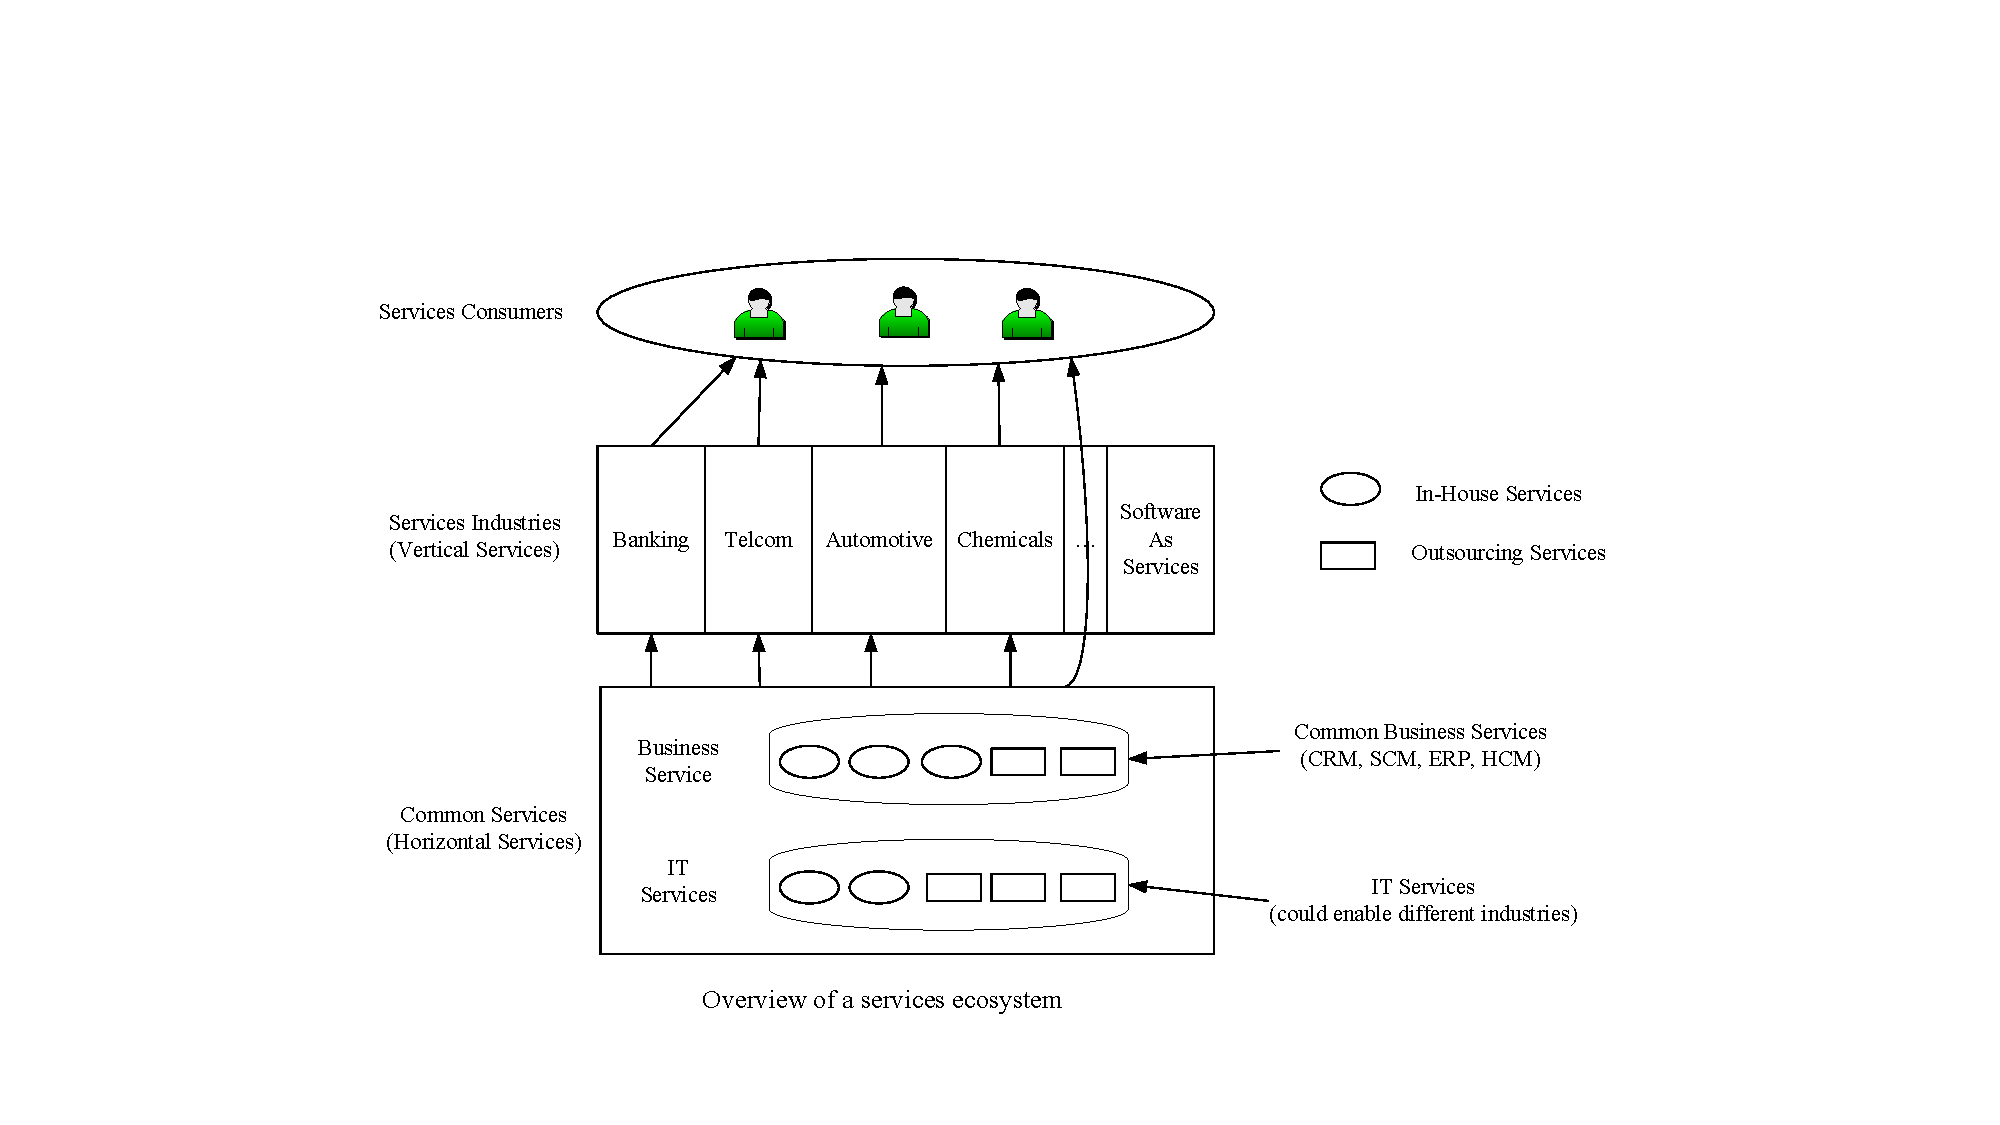
\includegraphics[width=0.85\textwidth]{images/Overview of a services ecosystem.pdf}
    \vspace{-1em}
\end{figure}

需要关注的问题有:
\vspace{-0.8em}
\begin{multicols}{2}
    \begin{itemize}[leftmargin=1em]
        \item 如何利用有限资源建立和维护适当的服务系统?
        \item 如何建立和维护适当的服务生态系统/服务库存?
    \end{itemize}   
\end{multicols}
\vspace{-1em}


\subsection{面向服务的范型}

\subsubsection{软件的发展过程}
\begin{itemize}
    \item 软件危机
    \vspace{-0.8em}
    \begin{multicols}{2}
    \begin{itemize}
        \item 用户需求不明确 
        \item 缺乏正确的理论指导
        \item 软件开发规模越来越大
        \item 软件开发复杂度越来越高 
    \end{itemize}  
    \end{multicols}
    \vspace{-1em}
    \item 服务系统的问题尤其突出
    \item 软件工程
    \vspace{-0.8em}
    \begin{multicols}{2}
    \begin{itemize}
        \item 软件过程及相关理论、方法和工具
        \item 软件产品簇、产品线
        \item \textbf{泛型}
    \end{itemize}  
    \end{multicols}
    \vspace{-1em}
\end{itemize}

\subsubsection{命令式(过程式)泛型}
\begin{wraptable}{r}{6cm}
    \centering
    \vspace{-5.5em}
    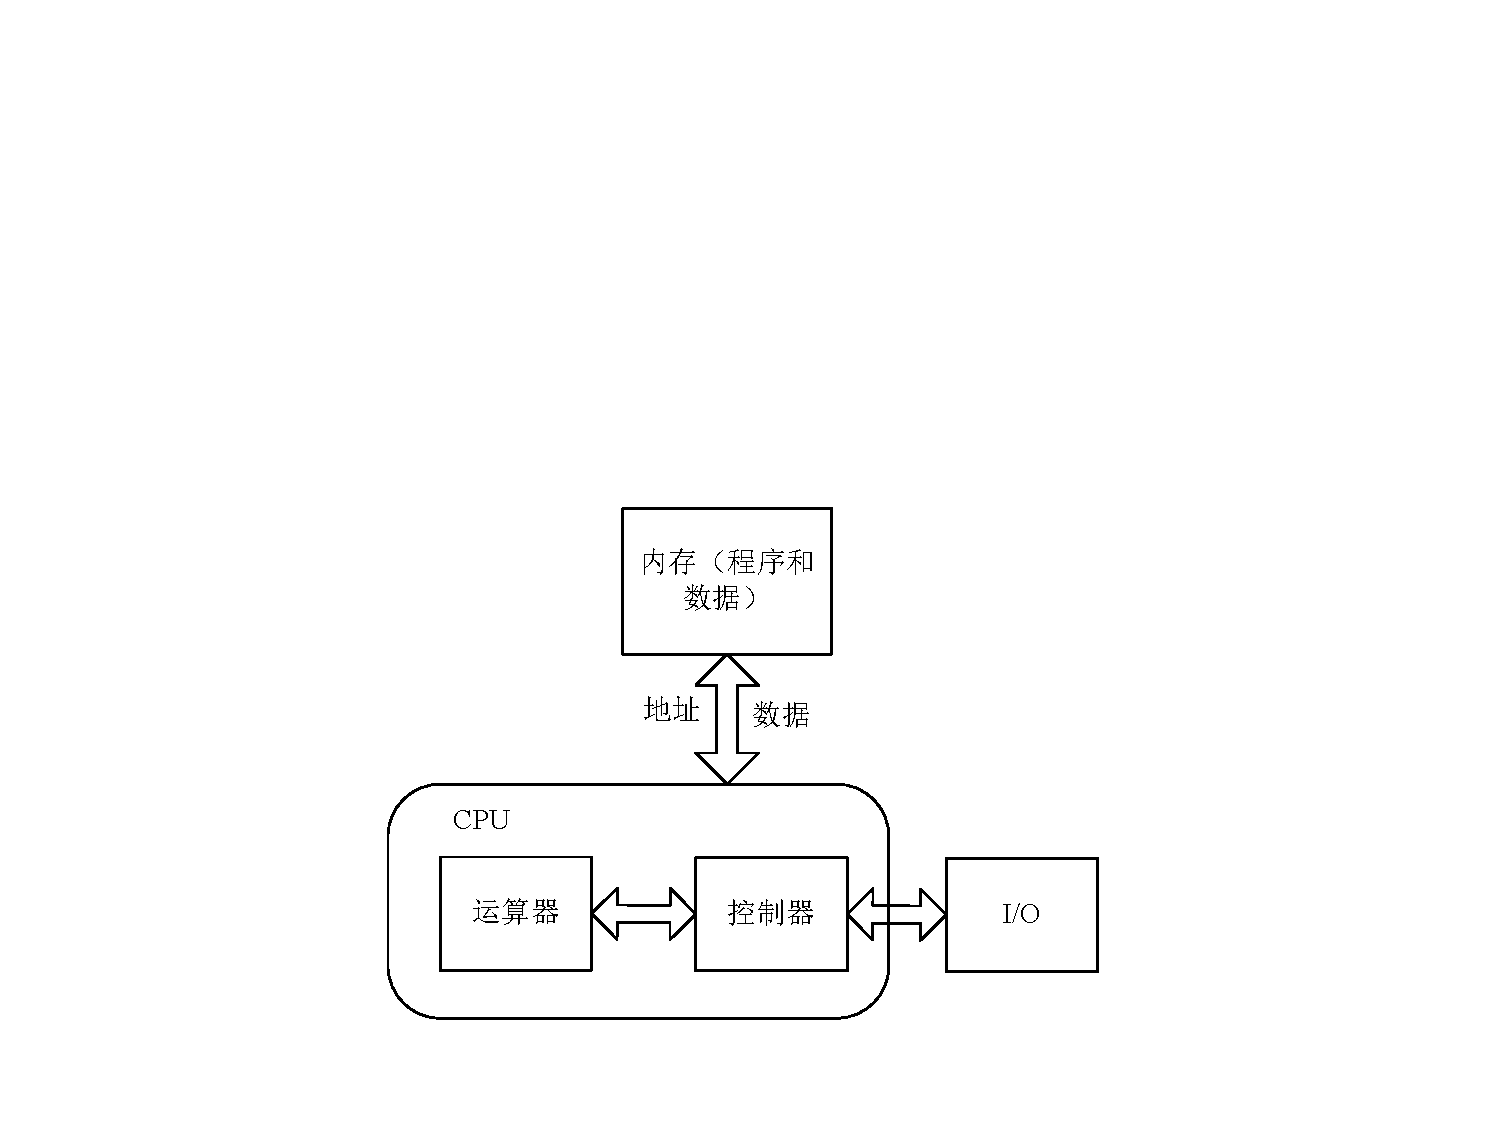
\includegraphics[width=6cm]{images/命令式(过程式)泛型.pdf}
    \vspace{-5em}
\end{wraptable}
用程序状态和改变程序状态的语句来描述计算

对冯·诺依曼式计算机的顺序执行机制的直接抽象

由过程完成复用

\subsubsection{面向对象的泛型}
\begin{itemize}
    \item 用封装了数据和操作的对象以及对象之间的消息传递描述计算
    \item 封装、继承、多态
\end{itemize}

\begin{figure}[H]
    \vspace{-0.5em}
	\centering
	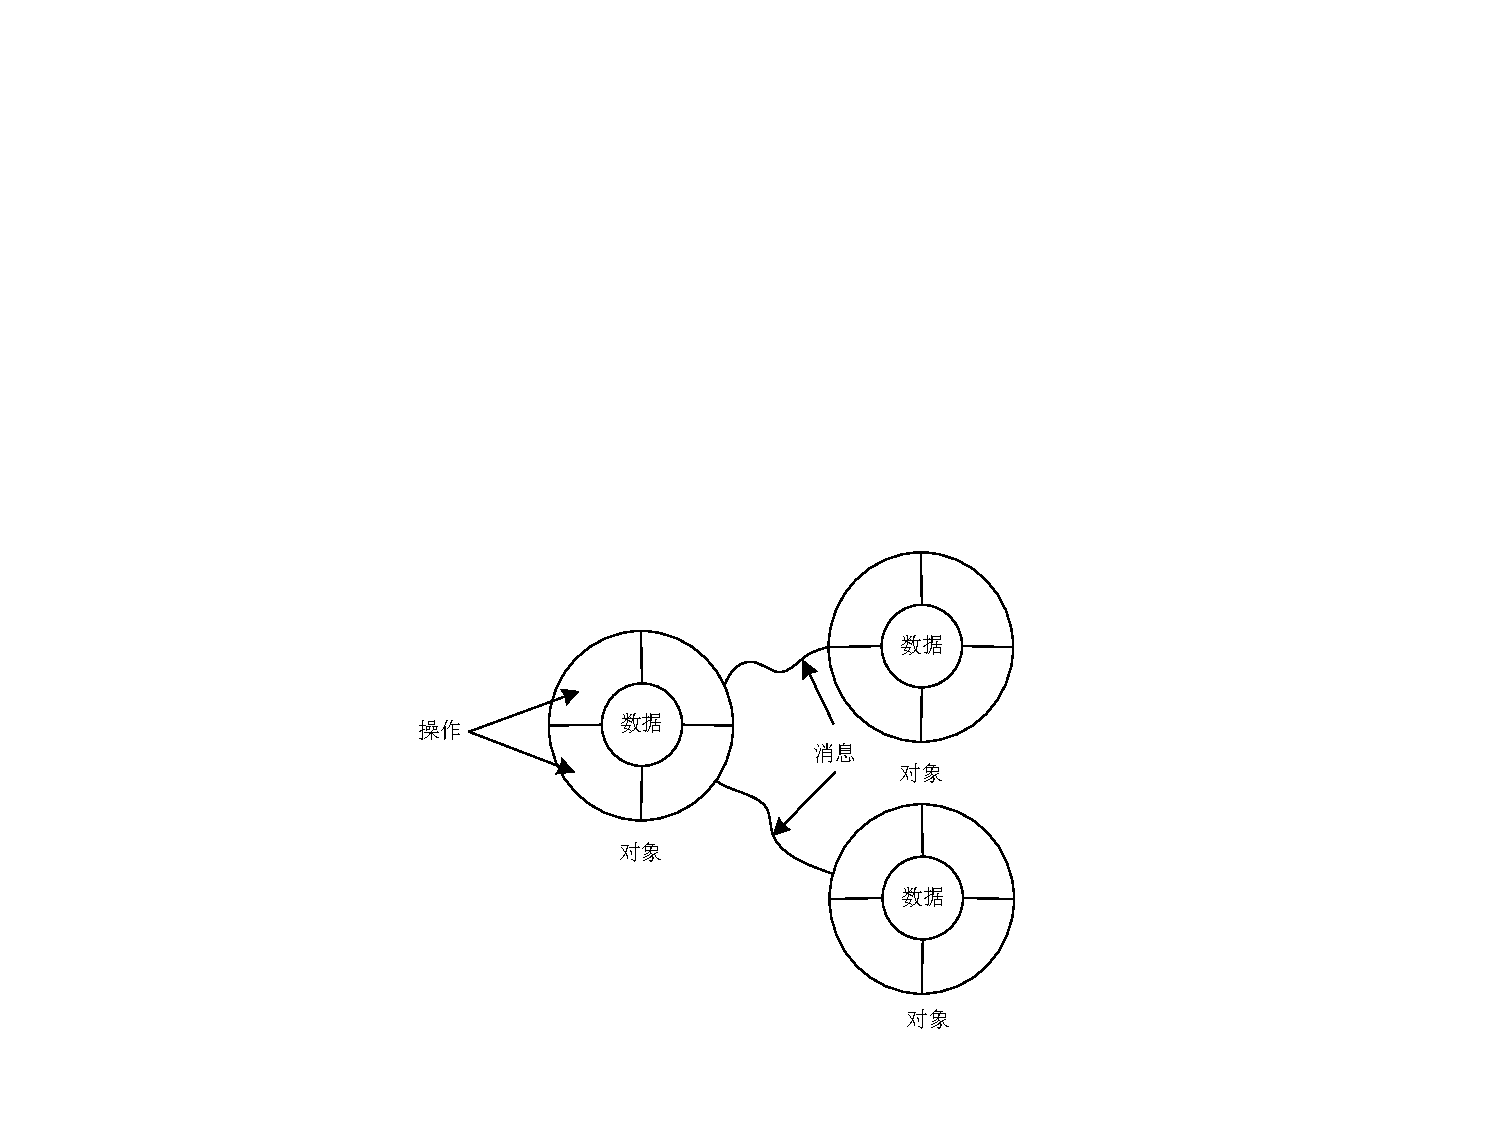
\includegraphics[width=0.45\textwidth]{images/面向对象的泛型.pdf}
    \vspace{-1em}
\end{figure}

\subsubsection{基于构件的泛型}
构件:模块化的、可部署、可替换的软件系统组成部分,它封装了内部的具体实现并对外提供统一接口。

以构建为基本单位进行分析和设计,整个软件的构造就被转换为:以构件的创建、构件的管理以及复用已有构件组装形成应用为基本活动。

\begin{spacing}{1}
    \begin{table}[H]
    \centering
    \begin{tabular}{|c|c|c|}
    \hline
                                                          & \textbf{基于构件}                                                                            & \textbf{面向对象}                                                                             \\ \hline
    抽象视角                                                  & \begin{tabular}[c]{@{}c@{}}构件是对客观世界的实体或者实体\\ 联合能提供的功能和服务的建模;\\ 仅仅关注实体的功能和服务\end{tabular} & \begin{tabular}[c]{@{}c@{}}对象是对客观世界基本实体的抽象,\\ 强调对实体的对应及对实体的建模;\\ 涉及实体的静态属性特征\end{tabular} \\ \hline
    \begin{tabular}[c]{@{}c@{}}可复用程度\\ 和复用机制\end{tabular} & 以组合的方式实现复用                                                                               & 以继承的方式实现复用                                                                                \\ \hline
    粒度不同                                                  & 大                                                                                        & 小                                                                                         \\ \hline
    \end{tabular}
\end{table}
\end{spacing}

\begin{figure}[H]
    \vspace{-0.5em}
	\centering
	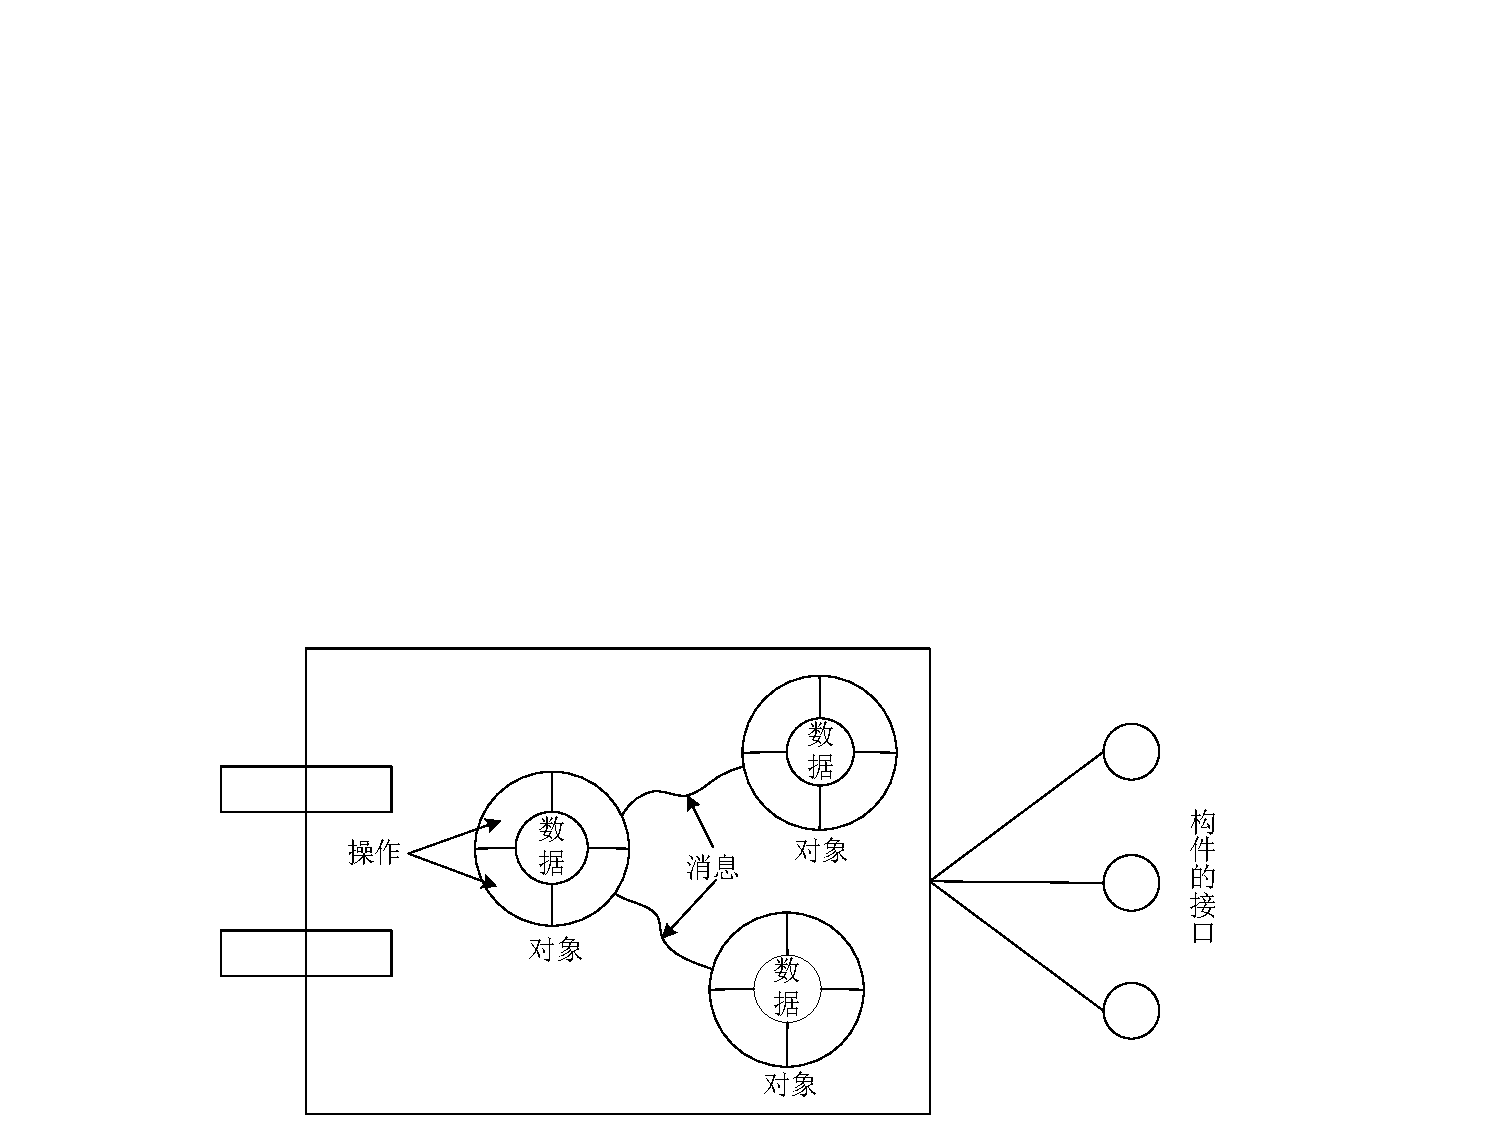
\includegraphics[width=0.65\textwidth]{images/基于构件与面向对象.pdf}
    \vspace{-1em}
\end{figure}

\subsubsection{面向服务的泛型}
\begin{itemize}
    \item 服务:是自治、开放、自描述、与实现无关的网络构件
    \begin{itemize}
        \item 自治:服务能够单独独立地完成一个任务(不依赖于其他构件,来完成它所需要完成的工作)
        \item 开放:对于构件而言,只要遵循了一般的协议或标准,当前服务的统一接口应该是跨公司、跨平台、全球范围之内可以相互调用的(进一步提升了它复用的可能性和范围)
        \item 自描述:服务应该自己能够描述自己完成的任务,而不应该有其他的附加手段去对于当前的服务来进行描述
        \item 与实现无关:只需提供统一接口,不用关心具体实现
    \end{itemize}
    \item 以服务的创建、服务的管理以及复用已有服务组装形成应用为基本活动
    \item 通过网络,使用标准方式互联
\end{itemize}

\begin{figure}[H]
    \vspace{-0.5em}
	\centering
	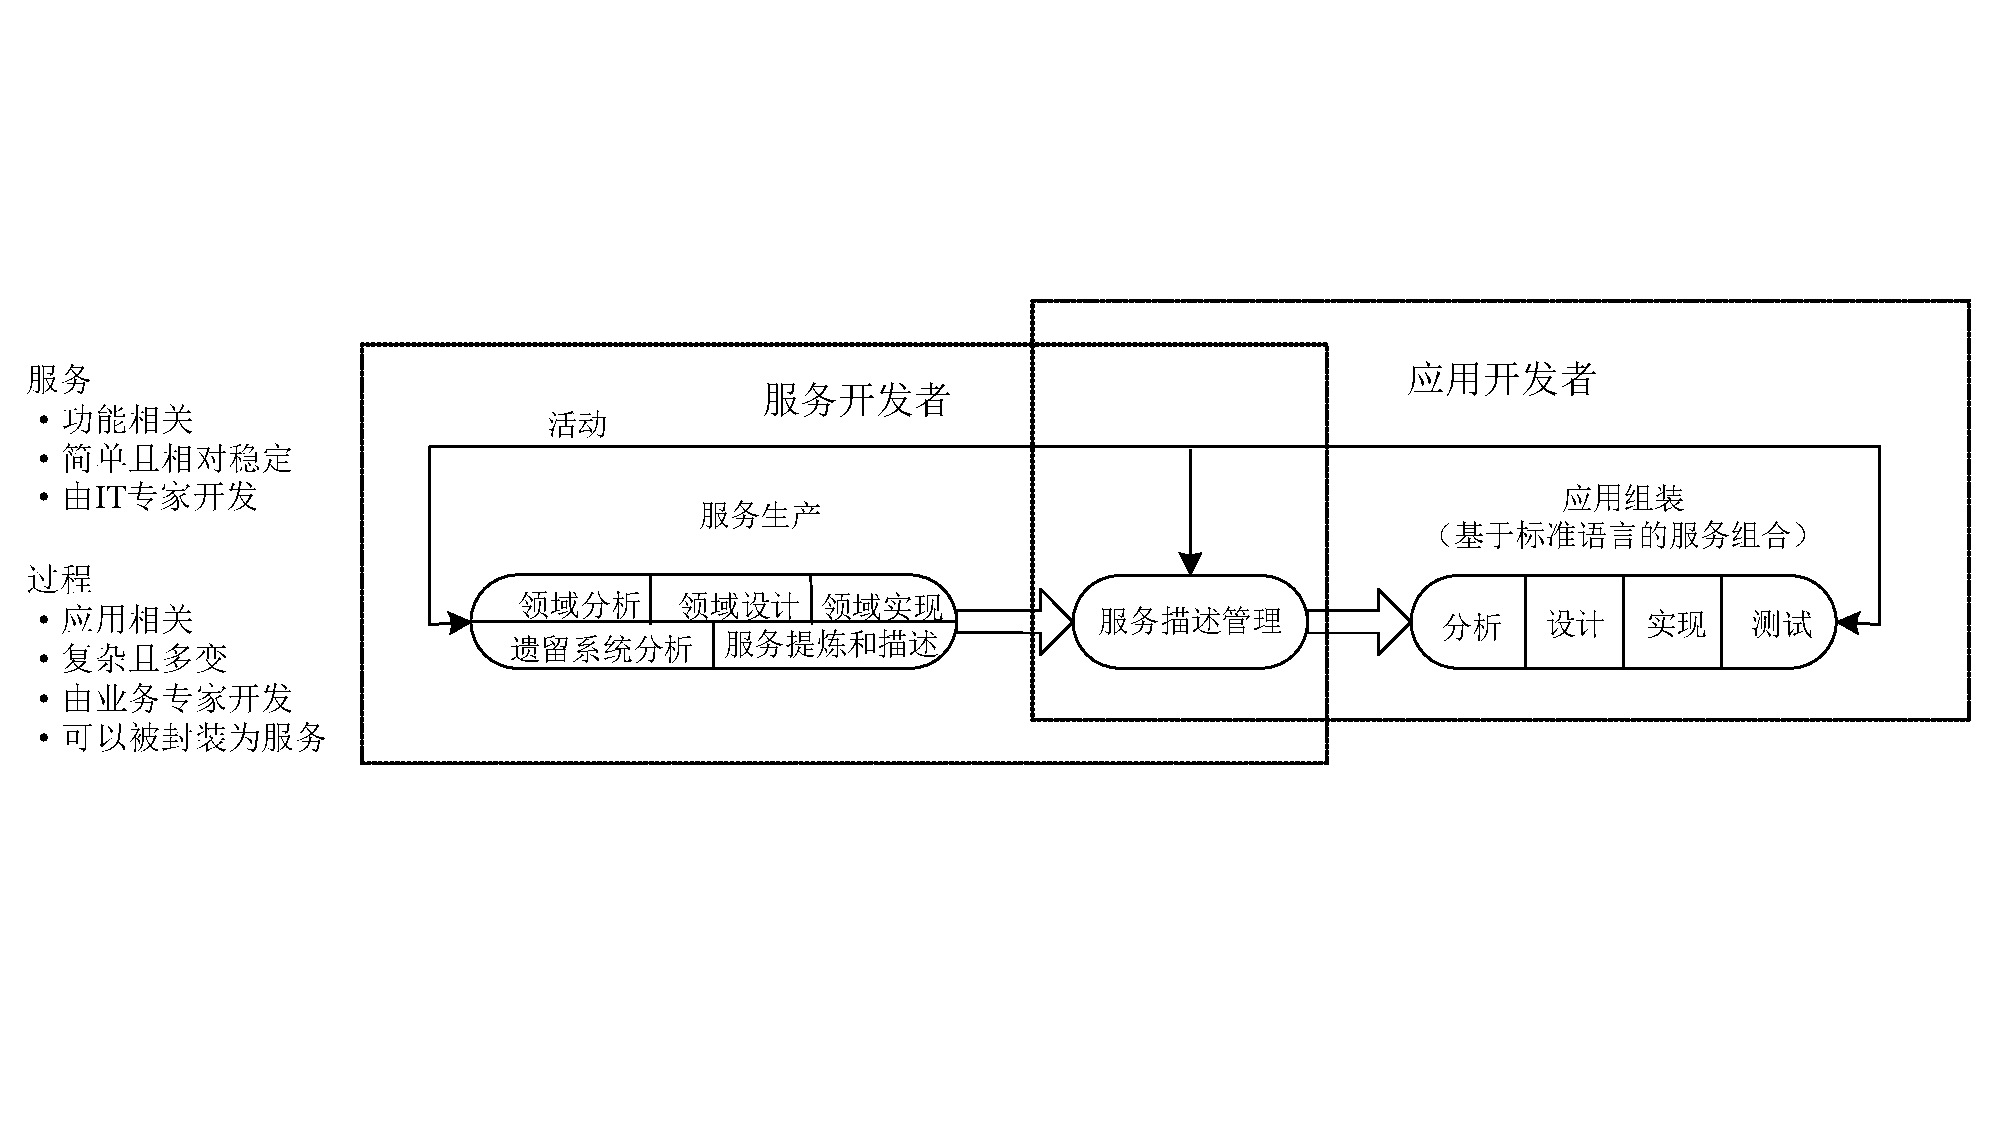
\includegraphics[width=\textwidth]{images/面向服务的泛型.pdf}
    \vspace{-1em}
\end{figure}

